\chapter{Schnyder woods}

\section{Canonical ordering}

\begin{defn}
	Given a plane triangulation (i.e., a non-crossing embedding of a triangulation in the plane, which means that the outerface is fixed) $G = (V, E)$, a canonical ordering of it is a numbering $1, 2, \dots, n$ of its vertices such that
	
	\begin{enumerate}[i)]
		\item the vertices of the outerface are $1, 2$ and $n = |V|$,
		\item for every $i = 3, 4, \dots, n - 1$,
		\begin{enumerate}[a)]
			\item the graph $G_i = G[1, 2, \dots, i]$ is vertex 2-connected,
			\item all vertices $j \leq i$ are drawn inside (or on the boundary) of the embedding of $G_i$ inherited from the embedding of $G$,
			\item all vertices $j > i$ are drawn outside the embedding of $G_i$ inherited from the embedding of $G$,
			\item the neighbors of vertex $i + 1$ in $G_i$ are lying consecutively on the boundary of $G_i$.
		\end{enumerate}
	\end{enumerate}
\end{defn}

\begin{thm}
	Every triangulation has a canonical ordering.
\end{thm}

\begin{proof}
	By induction from $n$ downto $3$, assign the numbers to the vertices. Once $n, n - 1, \dots, i + 1$ are assigned, choose as vertex $i$ such a vertex on the boundary of $G_i$ whose deletion from $G_i$ leaves $G_{i-1}$ vertex 2-connected. The only obstacle to preserving 2-connectedness is if $i$ would be incident to a diagonal edge (an edge with both end-vertices on the boundary of the outerface, but which itself is not a part of the boundary). But there is always a vertex which is not incident with any diagonal (to observe this, consider a vertex which is incident with a shortest possible diagonal, with the length of a diagonal being measured by the number of vertices of the boundary that it cuts off of $G_i$). So assign $i$ to a vertex (there may be more options) which is not incident to any diagonal. Then a), b) and c) are fulfilled for $G_{i-1}$. Note that d) follows from b) and c).
\end{proof}

\section{Schnyder woods}

\begin{algorithm}[!ht]
	\caption{Schnyder}
	\begin{algorithmic}[1]
		\Require A plane triangulation $G = (V, E)$ and a canonical ordering of it.
		\For{$i := 3 \dots n -1$}
			\State set $b(i)$ to be the leftmost neighbor of $i$ on the boundary of $G_{i-1}$, direct the edge $ib(i)$ in this direction and color it blue;
			\State set $g(i)$ to be the rightmost neighbor of $i$ on the boundary of $G_{i-1}$, direct the edge $ig(i)$ in this direction and color it green;
			\State set $r(i)$ to be the neighbor of $i$ with the highest number, direct the edge $ig(i)$ in this direction and color it red
		\EndFor
		\State \Return the orientation of $G$, the coloring of its edges and the mappings $b, g$ and $r$.
	\end{algorithmic}
\end{algorithm}

\begin{figure}[!ht]\centering
	\begin{subfigure}{0.45\textwidth}\centering
		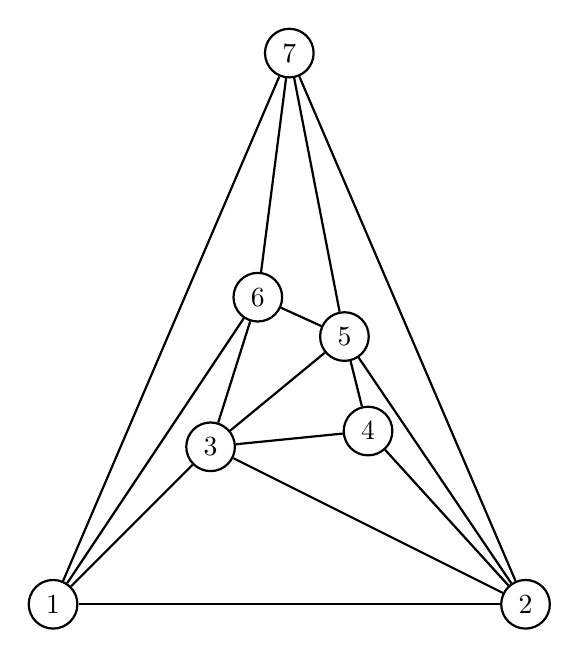
\begin{tikzpicture}[main/.style = {draw, circle, thick}]
			\node[main] (1) at (-1,-1) {1};
			\node[main] (2) at (5,-1) {2};
			\node[main] (3) at (1,1) {3};
			\node[main] (4) at (3, 1.2) {4};
			\node[main] (5) at (2.7, 2.4) {5};
			\node[main] (6) at (1.6, 2.9) {6};
			\node[main] (7) at (2, 6) {7};
			\draw[thick] (1) edge (3);
			\draw[thick] (1) edge (2);
			\draw[thick] (1) edge (7);
			\draw[thick] (1) edge (6);
			\draw[thick] (6) edge (3);
			\draw[thick] (4) edge (3);
			\draw[thick] (5) edge (3);
			\draw[thick] (2) edge (3);
			\draw[thick] (2) edge (4);
			\draw[thick] (2) edge (5);
			\draw[thick] (2) edge (7);
			\draw[thick] (5) edge (4);
			\draw[thick] (5) edge (6);
			\draw[thick] (7) edge (6);
			\draw[thick] (7) edge (5);
		\end{tikzpicture}
	\end{subfigure}
	\begin{subfigure}{0.45\textwidth}\centering
		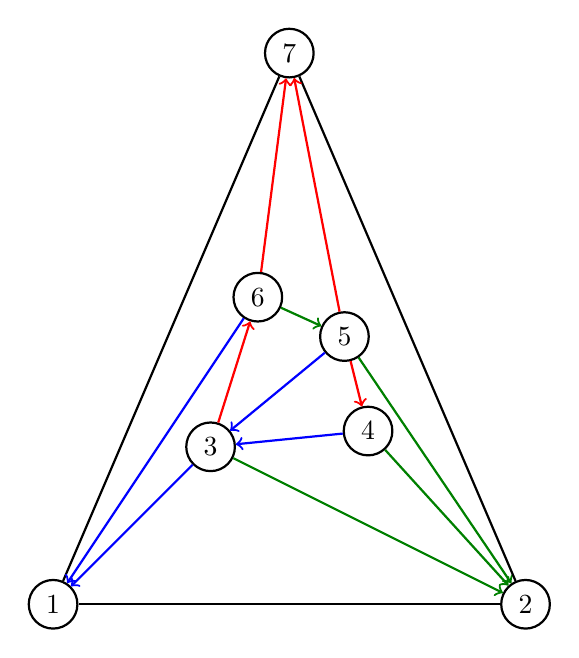
\begin{tikzpicture}[main/.style = {draw, circle, thick}]
			\node[main] (1) at (-1,-1) {1};
			\node[main] (2) at (5,-1) {2};
			\node[main] (3) at (1,1) {3};
			\node[main] (4) at (3, 1.2) {4};
			\node[main] (5) at (2.7, 2.4) {5};
			\node[main] (6) at (1.6, 2.9) {6};
			\node[main] (7) at (2, 6) {7};
			\draw[thick, ->, color=Blue] (3) edge (1);
			\draw[thick] (1) edge (2);
			\draw[thick] (1) edge (7);
			\draw[thick, ->, color=Blue] (6) edge (1);
			\draw[thick, ->, color=Red] (3) edge (6);
			\draw[thick, ->, color=Blue] (4) edge (3);
			\draw[thick, ->, color=Blue] (5) edge (3);
			\draw[thick, ->, color=Green] (3) edge (2);
			\draw[thick, ->, color=Green] (4) edge (2);
			\draw[thick, ->, color=Green] (5) edge (2);
			\draw[thick] (2) edge (7);
			\draw[thick, ->, color=Red] (5) edge (4);
			\draw[thick, ->, color=Green] (6) edge (5);
			\draw[thick, ->, color=Red] (6) edge (7);
			\draw[thick, ->, color=Red] (5) edge (7);
		\end{tikzpicture}
	\end{subfigure}
	\caption{An illustration to canonical orderings and Schnyder woods.}
\end{figure}

\begin{thm}
	The blue edges form a tree rooted in vertex 1 and spanning the vertices $1, 3, \dots, n - 1$, the green edges form a tree rooted in vertex 2 and spanning the vertices $2, 3, \dots, n - 1$, and the red edges form a tree rooted in vertex n and spanning the vertices $3, \dots , n$. Every edge of $G$, except of $12, 1n, 2n$, belongs to exactly one of these trees.
\end{thm}

\begin{proof}
	Clear from the construction and properties of canonical orderings.
\end{proof}

\begin{cor}
	The edges of a planar triangulation can be partitioned into edge sets of 3 trees and a triangle. Such a collection of three trees is called a \textbf{Schnyder wood} of $G$.
\end{cor}

\begin{figure}[!ht]\centering
	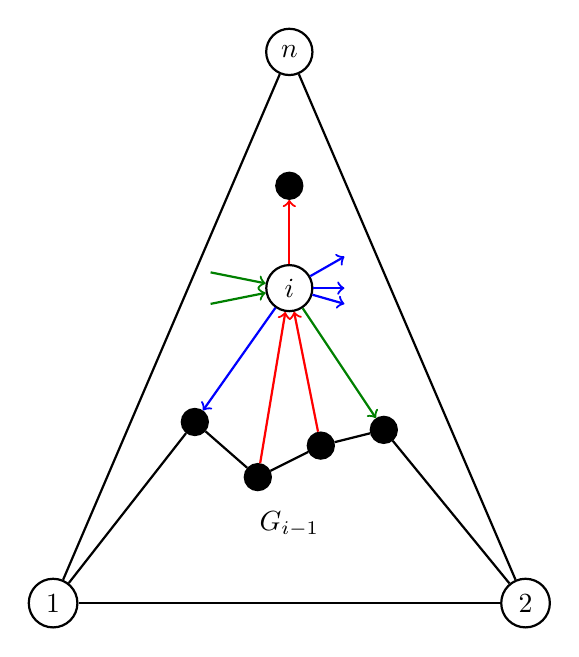
\begin{tikzpicture}[main/.style = {draw, circle, thick}]
		\node[main] (1) at (-1,-1) {1};
		\node[main] (2) at (5,-1) {2};
		\node[main, fill] (3) at (.8,1.3) {};
		\node[main, fill] (4) at (3.2, 1.2) {};
		\node[main, fill] (5) at (2.4, 1) {};
		\node[main, fill] (6) at (1.6, 0.6) {};
		\node[main] (n) at (2, 6) {$n$};
		\node[main] (i) at (2, 3) {$i$};
		\node[main, fill] (7) at (2, 4.3) {};
		\node (G) at (2, 0) {$G_{i-1}$};
		\draw[thick] (1) edge (3);
		\draw[thick] (1) edge (2);
		\draw[thick] (1) edge (n);
		\draw[thick] (6) edge (3);
		\draw[thick] (2) edge (4);
		\draw[thick] (2) edge (n);
		\draw[thick] (5) edge (4);
		\draw[thick] (5) edge (6);		
		\draw[thick, color=Blue, ->] (i) edge (3);
		\draw[thick, color=Red, ->] (6) edge (i);
		\draw[thick, color=Red, ->] (5) edge (i);
		\draw[thick, color=Green, ->] (i) edge (4);
		\draw[thick, color=Red, ->] (i) edge (7);
		\draw[thick, color=Green, ->] (1, 3.2) -- (i);
		\draw[thick, color=Green, ->] (1, 2.8) -- (i);
		\draw[thick, color=Blue, ->] (i) -- (2.7, 3.4);
		\draw[thick, color=Blue, ->] (i) -- (2.7, 2.8);
		\draw[thick, color=Blue, ->] (i) -- (2.7, 3);
	\end{tikzpicture}
	\caption{The rotation scheme of incoming and outgoing edges around a vertex in the Schnyder wood.}
\end{figure}

\begin{prop}
	Locally around every inner vertex of $G$, we see (in the counter-clock-wise order) one outgoing blue edge, several (or none) incoming red edges, one outgoing green edge, several (or none) incoming blue edges, one outgoing red edge, and several (or none) incoming green edges.
\end{prop}

\section{Triangle contact representations}

\begin{thm}[de Fraysseix, Ossona de Mendez, Rosenstiehl]
	Every planar graph is a contact graph of isosceles triangles with horizontal bases.
\end{thm}

\begin{proof}
	It suffices to prove the theorem for triangulations, since every planar graph is an induced subgraph of a triangulation. Given a triangulation $G = (V, E)$, fix an embedding and consider a canonical ordering with respect to this embedding, and run algorithm Schnyder on this canonical ordering. Draw $n + 1 = |V| + 1$ parallel horizontal lines and build triangles as follows:
	
	\begin{enumerate}
		\item Triangle $T_i$ is isosceles and its base lies on the $i$-th line,
		\item The peaks of $T_1$ and $T_2$ are on the $(n + 1)$-st line, the left corner of $T_2$ touches the right side of $T_1$,
		\item For every $i = 1, 2, \dots, n$, the left corner of $T_i$ lies on the right side of $T_{b(i)}$, the right corner of $T_i$ lies on the left side of $T_{g(i)}$ and the peak of $T_i$ lies on the $r(i)$-th line (on the $(n + 1)$-st line for $i = n$).
	\end{enumerate}
	
	Construct the triangles from $T_1$ to $T_n$. For $T_1$, only the lines supporting its base and peak are prescribed, the triangle is free otherwise. For $T_2$, the freedom is restricted only to the position of the right corner (which then determines the position of the peak). For $i > 2$, the triangles are then determined uniquely. The loop invariant of this inductive construction is that for $i > 1$, the upper boundary of the union of triangles $T_1 , T_2 , \dots, T_i$ is connected and the order in which the triangles appear on this boundary is the same as the order of the corresponding vertices appearing on the upper boundary of $G_i$. This implies that $T_i$ is always placed in the way that it is touching the respective neighbors, but not crossing any triangle of the representation.
\end{proof}

\begin{figure}
	\begin{subfigure}{0.45\textwidth}\centering
		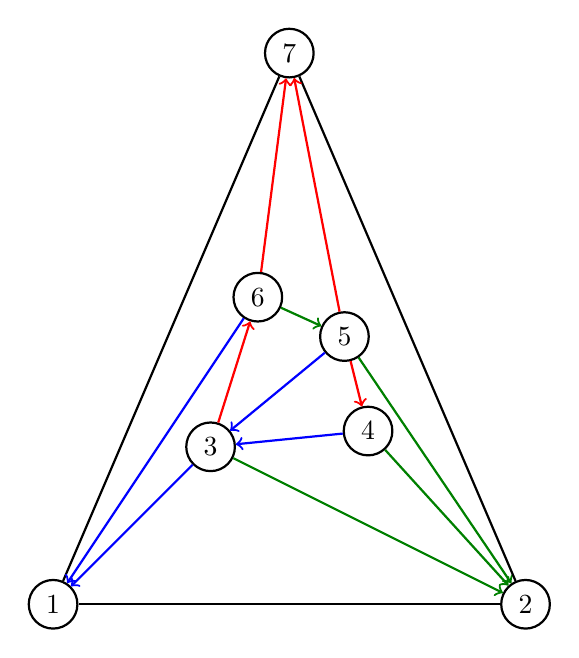
\begin{tikzpicture}[main/.style = {draw, circle, thick}]
			\node[main] (1) at (-1,-1) {1};
			\node[main] (2) at (5,-1) {2};
			\node[main] (3) at (1,1) {3};
			\node[main] (4) at (3, 1.2) {4};
			\node[main] (5) at (2.7, 2.4) {5};
			\node[main] (6) at (1.6, 2.9) {6};
			\node[main] (7) at (2, 6) {7};
			\draw[thick, ->, color=Blue] (3) edge (1);
			\draw[thick] (1) edge (2);
			\draw[thick] (1) edge (7);
			\draw[thick, ->, color=Blue] (6) edge (1);
			\draw[thick, ->, color=Red] (3) edge (6);
			\draw[thick, ->, color=Blue] (4) edge (3);
			\draw[thick, ->, color=Blue] (5) edge (3);
			\draw[thick, ->, color=Green] (3) edge (2);
			\draw[thick, ->, color=Green] (4) edge (2);
			\draw[thick, ->, color=Green] (5) edge (2);
			\draw[thick] (2) edge (7);
			\draw[thick, ->, color=Red] (5) edge (4);
			\draw[thick, ->, color=Green] (6) edge (5);
			\draw[thick, ->, color=Red] (6) edge (7);
			\draw[thick, ->, color=Red] (5) edge (7);
		\end{tikzpicture}
	\end{subfigure}
	\begin{subfigure}{0.45\textwidth}\centering
		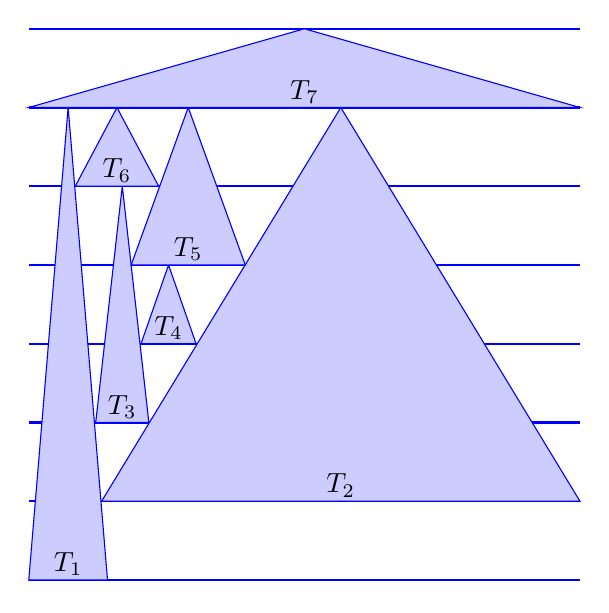
\begin{tikzpicture}
			\draw[Blue, thick] (0,0) -- (7,0);
			\draw[Blue, thick] (0,1) -- (7,1);
			\draw[Blue, thick] (0,2) -- (7,2);
			\draw[Blue, thick] (0,3) -- (7,3);
			\draw[Blue, thick] (0,4) -- (7,4);
			\draw[Blue, thick] (0,5) -- (7,5);
			\draw[Blue, thick] (0,6) -- (7,6);
			\draw[Blue, thick] (0,7) -- (7,7);
			\draw[Blue, fill=Blue!20] (0,0) -- (1,0) -- (0.5,6) -- cycle;
			\draw[Blue, fill=Blue!20] (0.925,1) -- (7,1) -- (3.9625,6) -- cycle;
			\draw[Blue, fill=Blue!20] (0.85,2) -- (1.525,2) -- (1.1875,5) -- cycle;
			\draw[Blue, fill=Blue!20] (1.425,3) -- (2.125,3) -- (1.775,4) -- cycle;
			\draw[Blue, fill=Blue!20] (1.3,4) -- (2.75,4) -- (2.025,6) -- cycle;
			\draw[Blue, fill=Blue!20] (0.59,5) -- (1.65,5) -- (1.12,6) -- cycle;
			\draw[Blue, fill=Blue!20] (0,6) -- (7,6) -- (3.5,7) -- cycle;
			\node at (.5, .2) {$T_1$};
			\node at (3.9625, 1.2) {$T_2$};
			\node at (1.1875, 2.2) {$T_3$};
			\node at (1.775, 3.2) {$T_4$};
			\node at (2.025, 4.2) {$T_5$};
			\node at (1.12, 5.2) {$T_6$};
			\node at (3.5, 6.2) {$T_7$};
		\end{tikzpicture}
	\end{subfigure}
	\caption{An illustration to contact representations by isosceles triangles.}
\end{figure}

\section{Drawing planar graphs on small grids}

\begin{thm}
	Every planar $n$-vertex graph allows a straight-line non-crossing embedding on a grid of size $n \times n$.
\end{thm}

\begin{proof}
	It suffices to prove the theorem for planar triangulations. Given a triangulation $G = (V, E)$, fix an embedding and consider a canonical ordering with respect to this embedding, and run algorithm Schnyder on this canonical ordering. Assign barycentric coordinates $(x_i , y_i , z_i)$ to every vertex $i = 3, 4, \dots, n - 1$ as follows (see Fig. \ref{coord} for illustration): The triangle $12n$ is divided into three regions by the blue, green and red directed paths from $i$ to the roots of the trees in the Schnyder wood. Let $x_i$ be the number of vertices in the region bounded by the blue and green paths and the side $12$, with the vertices on the green path being counted in, but not the vertices of the blue path. Similarly, $y_i$ is the number of vertices in the region bounded by the blue and red paths and the side $1n$, with the vertices on the blue path being counted in, but not the vertices of the red path, and $z_i$ is the number of vertices in the region bounded by the red and green paths and the side $n2$, with the vertices on the red path being counted in, but not the vertices of the green one. Vertex $i$ itself is not counted in neither of the regions.

	\begin{figure}[!ht]\centering
		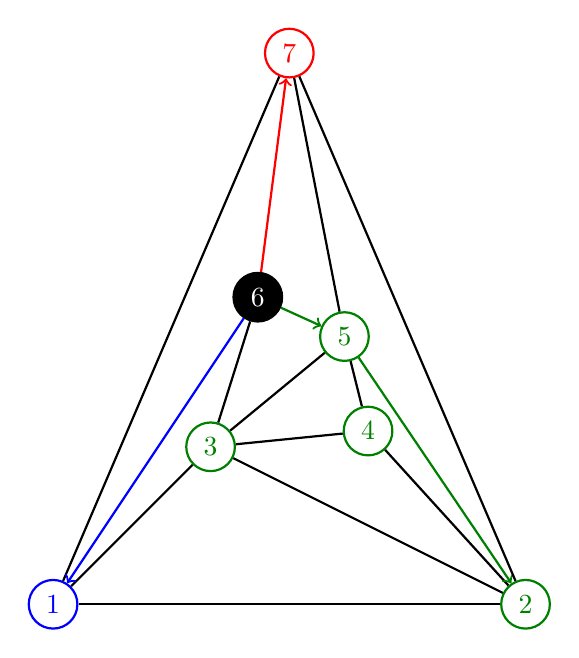
\begin{tikzpicture}[main/.style = {draw, circle, thick}]
			\node[main, Blue] (1) at (-1,-1) {1};
			\node[main, Green] (2) at (5,-1) {2};
			\node[main, Green] (3) at (1,1) {3};
			\node[main, Green] (4) at (3, 1.2) {4};
			\node[main, Green] (5) at (2.7, 2.4) {5};
			\node[main, fill, Black] (6) at (1.6, 2.9) {\textcolor{white}{6}};
			\node[main, Red] (7) at (2, 6) {7};
			\draw[thick] (1) edge (3);
			\draw[thick] (1) edge (2);
			\draw[thick] (1) edge (7);
			\draw[thick, color=Blue, ->] (6) edge (1);
			\draw[thick] (6) edge (3);
			\draw[thick] (4) edge (3);
			\draw[thick] (5) edge (3);
			\draw[thick] (2) edge (3);
			\draw[thick] (2) edge (4);
			\draw[thick, color=Green, ->] (5) edge (2);
			\draw[thick] (2) edge (7);
			\draw[thick] (5) edge (4);
			\draw[thick, color=Green, ->] (6) edge (5);
			\draw[thick, color=Red, ->] (6) edge (7);
			\draw[thick] (7) edge (5);
		\end{tikzpicture}
		\caption{An illustration to the definition of barycentric coordinates from Schnyder woods. The green vertices are counted for the definition of $x_6$, the blue one for the definition of $y_6$ and the red one for the definition of $z_6$. Vertex 6 itself does not contribute to any of the coordinates.}
		\label{coord}
	\end{figure}

	Then every vertex except of $i$ belongs to exactly one of the regions, end hence
	
	$$
	x_i + y_i + z_i = n - 1
	$$
	
	for every $i$. For $i = 1, 2$, and $n$, we set
	
	$$
	\begin{array}{lll}
		x_1 = 0,   &y_1 = 0,   &z_1 = n - 1\\
		x_2 = 0,   &y_2 = n-1, &z_2 = 0\\
		x_n = n-1, &y_n = 0,   & z_n = 0 	
	\end{array}
	$$
	
	Place vertex $i$ in the point with barycentric coordinates $(x_i , y_i , z_i)$ in a triangular $n \times n \times n$ grid (the lines of the grid have coordinates $0, 1, \dots, n - 1$). Draw the edges of $G$ as straight-line segments
	connecting their vertices.
	
	\begin{claim}
		Consider a vertex $i \in \{3, 4, \dots, n - 1\}$. In the drawing constructed as above, the blue edge $ib(i)$ is directed into the bottom-left sextant of $i$, the edge $ig(i)$ is directed into the bottom-right sextant of $i$, and the edge $ir(i)$ is directed into the top sextant of $i$.
		\label{claim-1}
	\end{claim}
	
	\begin{proof}[Proof of claim]
		From the definition of the coordinates, it follows that $xb(i) \leq x_i$, $yb(i) < y_i$ and $zb(i) \geq z_i$, and this implies the direction of the edge $ib(i)$. Similarly for the others.
	\end{proof}
	
	\begin{claim}
		The rotation scheme of the edges around each vertex $i$ in the barycentric drawing is the same as the rotation scheme of the edges incident to the same vertex in $G$.
	\end{claim}
	
	\begin{proof}[Proof of claim]
		This follows by application of Claim \ref{claim-1} to the other end-vertices of the edges directed into $i$.
	\end{proof}
	
	\begin{claim}
		The barycentric drawing is non-crossing and topologically equivalent to the plane embedding of $G$ we started with.
	\end{claim}
	
	\begin{proof}[Proof of claim]
		If the rotation schemes for all vertices of drawings of two 3-connected graphs are the same and one of the drawings is non-crossing, then so is the other one, and the drawings are topologically equivalent.
	\end{proof}
\end{proof}

\section{Boxicity of graphs}

\begin{defn}
	The \textbf{boxicity} of a graph $G$, denoted by $\text{box}(G)$, is the smallest integer $d$ such that $G$ is an intersection graph of boxes in $\R^d$ (i.e., of $d$-dimensional intervals in the $d$-dimensional Euclidean space).
\end{defn}

\begin{prop}
For every graph $G = (V, E)$, its boxicity is a correctly defined finite number. It equals the minimum number of interval graphs whose intersection is equal to $G$, i.e., the minimum number $d$ for which sets $E_i \subseteq \binom{V}{2} , i = 1, 2, \dots, d$ exist, such that $E = \cup_{i=1}^d E_i$ and $(V, E_i)$ is an interval graph for every $i = 1, 2, \dots, d$.
\end{prop}

\begin{proof}
	An exercise. Proof the claim for graphs $G$ which are not complete. For a complete graph, the boxicity is $0$, which corresponds to the fact that the intersection of an empty set of subsets of a ground set ($E$, in this case) is by default set to be equal to the ground set itself.
\end{proof}

\section{Grid intersection graphs}

\begin{defn}
	A graph is a \textbf{Grid Intersection graph} if it has an intersection representation by vertical and horizontal segments in which no two segments of the same direction share a point (in other words, all vertical, as well as all horizontal, segments are pairwise disjoint).
\end{defn}

It is easy to observe that every grid intersection graph has a grid intersection representation in which no two segments lie on the same line. Moreover, the exact $x$-coordinates of the vertical segments, nor the exact $y$-coordinates of the horizontal ones, are important, only their linear orders. Thus we assume that our bipartite graph $G = (A \cup B, E)$ has its vertices linearly ordered within the classes of bipartition, $A = \{a_1 , a_2 , \dots, a_n\}, B = \{b_1 , b_2 \dots, b_m\}$. We further assume that the vertices of $A$ are to be represented by vertical segments and the vertices of $B$ by horizontal ones. We say that a grid intersection representation respects the orders of $A$ and $B$ if for every $i < j$, the $x$-coordinate of $a_i$ is smaller than the $x$-coordinate of $a_j$, and the $y$-coordinate of $b_i$ is smaller than the $y$-coordinate of $b_j$.

\begin{thm}
	The graph $G = (A \cup B, E)$ has a grid intersection representation that respects the linear orders of $A$ and $B$ if and only if there are no 6 indices $i < j < k, \alpha < \beta < \gamma$ such that $a_i b_\beta , a_k b_\beta , a_j b_\alpha , a_j b_\gamma$ are edges of $G$ and $a_j b_\beta$ is not. Such a configuration of 6 vertices is called a \textbf{volswagen} in $G$.
	\label{thm-5}
\end{thm}

\begin{proof}
	Exercise.
\end{proof}

It is easy (i.e., decidable in polynomial time) to check if a bipartite graph contains a volkswagen with respect to given linear orderings of the vertices in its classes of bipartition. We will see in the last class that it is NP-complete to decide if a given bipartite graph is a grid intersection graph, which means that it is NP-complete to decide if a given bipartite graph allows linear orderings of its classes of bipartition with respect to which there is no volkswagen. The following problem is thus quite interesting in this context.

\textbf{Open problem:} Given a bipartite graph with one class of bipartition linearly ordered. How difficult is to decide if the other class of bipartition can be linearly ordered so that there is no volkswagen with respect to these orderings?

\begin{thm}[Bellantoni, Hartman, Przytycka, Whitesides]
	Every bipartite graph of boxicity $2$ is a grid intersection graph.
\end{thm}

\begin{figure}[!ht]\centering
	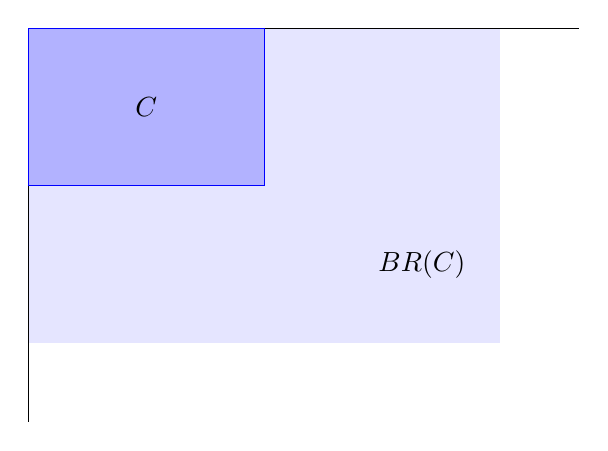
\begin{tikzpicture}
		\draw[black!0, fill=blue!10] (0,-2) rectangle (6,2);
		\draw (0,2) -- (7,2);
		\draw (0,2) -- (0, -3);
		\draw[blue, fill=blue!30] (0,0) rectangle (3,2);
		\node at (1.5, 1) {$C$};
		\node at (5,-1) {$BR(C)$};
	\end{tikzpicture}
	\caption{An illustration to the definition of region $BR(C)$.}
\end{figure}

\begin{proof}[Sketch of proof]
	Suppose $G = (A \cup B, E)$ is a bipartite graph and let $\mathcal{R} = \{R(u) : u \in A \cup B\}$ be an intersection representation of $G$ by axes-parallel rectangles in the plane. For a rectangle $C$ in the plane, we define regions $BL(C)$, $BR(C)$, $TL(C)$, $TR(C)$ as follows: $BR(C)$ contains all points with $x$-coordinate greater than the $x$-coordinate of the left side of $C$, with $y$-coordinate smaller than the $y$-coordinate of the top side of $C$, but which do not lie inside the rectangle $C$. The other regions ($BL$ standing for Bottom-Left, $TL$ standing for Top-Left, and $TR$ standing for Top-Right) are defined in a similar way. Then define two binary relations, one on $A$, the other one on $B$, as follows
	
	$$
	\begin{array}{c c c c}
		a_1 <_R a_2 & \Leftrightarrow & R(a_1) \cap BR(R(a_2)) \neq \emptyset & \text{ for } a_1, a_2 \in A, \\
		b_1 <_R b_2 & \Leftrightarrow & R(b_1) \cap BL(R(b_2)) \neq \emptyset & \text{ for } b_1, b_2 \in B. \\
	\end{array}
	$$
	
	\begin{claim}
		Both relations $<_R$ and $<_L$ are antireflexive, antisymmetric and acyclic. It follows that the transitive closures $<_{R}^T$ and $<_{L}^T$ of $<_R$ and $<_L$, respectively, are partial orders.
	\end{claim}
	
	Let $<_R^\ast$ and $<_L^\ast$ be topological sortings of $<_R^T$ and $<_L^T$, respectively.
	
	\begin{claim}
		With respect to the linear orderings $<_R^\ast$ and $<_L^\ast$ of its classes of bipartition, $G$ has no volkswagens. Hence $G$ has a grid intersection representation respecting these orders by Theorem \ref{thm-5}.
	\end{claim}
\end{proof}